\chapter{Related work}\label{sec:rel}
This chapter reviews related work on the \emph{realisability problem} for
\emph{global types}, both within the same theoretical framework and in
closely related models.  
Our approach adopts a definition of global types that captures a set of
MSCs, following a line of research initiated in~\cite{di2023partial} and
extended in~\cite{di2025realisability}, which aims to establish a
general framework for communication semantics.  
We first discuss these foundational works to situate our own
contributions.  
We then examine recent advances by
Stutz~et~al.~\cite{stutz2024implementability}, who provide a
comprehensive automata-theoretic treatment of the realisability problem,
and trace this line of inquiry back to early results by
Alur~et~al.~\cite{alur2000inference} and
Lohrey~et~al.~\cite{lohrey2003realizability}.  
Finally, we consider related formalisms such as Multiparty Session Types
(MPST) and Choreography Automata~\cite{barbanera2020choreography},
highlighting conceptual connections and key differences with the
approach developed in this thesis.

\section{Hierarchy of communication model's semantics}\label{sec:hier}
We defined early some communication semantics of out interest, informally, 
in Chapter~\ref{chap:intro} and, formally, the $\synchmodel$ 
in Definition~\ref{def:synchronous}.
Furthermore, \cite{di2023partial} show some other interesting 
semantics. It also introduces a hierarchy of communication
semantics, illustrated in Figure~\ref{fig:coms}. The main objective of
this work was to establish a hierarchy that preserves \emph{monotonic}
properties: if a property holds for a given communication semantic, it
should also hold for all semantics contained within it. However, it was
shown that this monotonicity only applies to specific properties, such
as \emph{weak-$k$-synchronizability}. In contrast, it does not generally
extend to the realisability problem, that is why we focused in particular
on certain semantics. We define subsequently some other useful and
well known communication semantics.

\bigskip

\begin{figure}[!ht]
\centering
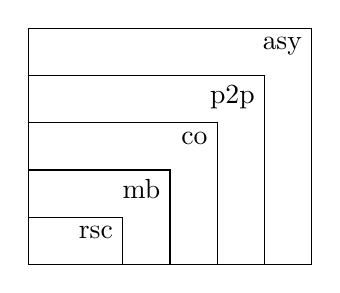
\begin{tikzpicture}[scale=0.6]
  % list of labels in order (from smallest to largest)
%   \def\labels{{rsc,nn,onen,mb,co,p2p,asy}}
  % loop to draw nested squares
  \foreach [count=\i] \lab in {rsc,mb,co,p2p,asy} {
    \draw (0,0) rectangle (\i+1,\i);
    \node[anchor=north east] at (\i+1,\i) {\lab};
  }
\end{tikzpicture}
\caption{Hierarchy of communication model semantics.}
\label{fig:coms}
\end{figure}

% A p2p-MSC is an MSC $M = (E,\to, \lhd, \lambda)$ where, for any two send events $s$ 
% and $s'$ such that $\lambda(s) \in \text{send}(p, q, \_), \lambda(s') in \text{send}(p, q, \_)$, 
% and $s \to^+ s'$, one of the following holds:
% - either $s, s' \in \text{matched}(M)$ with $s \lhd r$ and $s' \lhd r'$ and 
% $r \to^+ r'$,
% - or $s' \in \text{unmatched}(M)$.
% Note that we cannot have two messages $m 1$ and $m 2$, both sent by $p$ to $q$, 
% in that order, such that $m 1$ is unmatched and $m 2$ is matched; unmatched 
% message $m 1$ excludes the reception of any later message.

\paragraph{Causally ordered}
In the causally ordered (\verb|co|) communication model, messages are delivered 
to a process in accordance with the causal dependencies of their emissions. 
In other words, if there are two messages $m_1$ and $m_2$ with the same recipient, 
such that there exists a causal path from $m_1$ to $m_2$, then $m_1$ must be received 
before $m_2$. This notion of causal ordering was first introduced by Lamport under the 
name ``happened-before'' relation. In Figure~\ref{fig:p2p}, this 
causality is violated: $m_1$ should be received before $m_3$. Causal delivery 
is commonly implemented using Lamport's logical clock algorithm \cite{lamport2019time}.

% An MSC $M = (E, \to, \lhd, \lambda)$ is causally ordered if, for any two send $s$ and 
% $s'$, such that $\lambda(s) \in \text{send}(\_, q, \_), \lambda(s') \in \text{send}(\_, q, \_)$, and 
% $s \leq_{\text{hb}} s'$:
% - either $s, s' \in \text{matched}(M)$ and $r \to^* r'$, with $r$ and $r'$ receive 
% events such that $s \lhd r$ and $s' \lhd r'$.
% - or $s' \in \text{unmatched}(M)$.

% Note that in a \verb|co|-MSC we cannot have two send events $s$ and $s'$ addressed 
% to the same process, such that $s$ is unmatched, $s'$ is matched, and 
% $s \leq_{\text{hb}} s'$.

\paragraph{Mailbox}
In this model, any two messages sent to the same process, regardless of the sender, 
must be received in the same order as they are sent. If a process receives $m_1$ 
before $m_2$, then $m_1$ must have been sent before $m_2$. \verb|mb| coordinates all 
the senders of a single receiver. This model is also called FIFO $n-1$.
In Figure~\ref{fig:mailbox}, an example for this communication model is shown.

\begin{figure}[!ht]
	\centering
	\begin{msc}[draw frame=none, draw head=none, msc keyword=, 
				head height=0px, label distance=0.5ex, 
				foot height=0px, foot distance=0px]{}
		\declinst{p}{p}{}
		\declinst{q}{q}{}
		\declinst{r}{r}{}
		\declinst{s}{s}{}

		\mess[pos=0.1]{$m_4$}{p}{s}[4]
		\nextlevel
		\mess[pos=0.8]{$m_1$}{p}{q}
		\nextlevel
		\mess[pos=0.2]{$m_2$}{r}{q}
		\nextlevel
		\mess[pos=0.8]{$m_3$}{r}{s}
	\end{msc}
	\caption{An example of mailbox semantic.}
	\label{fig:mailbox}
\end{figure}

% An MSC $M = (E, \to, \lhd, \lambda)$ is a \verb|mb|-MSC if it has a linearization 
% $\rightsquigarrow$ where, for any two send events $s$ and $s'$, such 
% that $\lambda (s) \in \text{send}(\_,q,\_), \lambda (s') \in \text{send}(\_,q,\_)$, and 
% $s \rightsquigarrow s'$
% - either $s,s' \in \text{matched}(M)$ and $r \rightsquigarrow r'$, where 
% $s \lhd r$ and $s' \lhd r'$,
% - or $s' \in \text{unmatched}(M)$.

% \paragraph{FIFO 1-n}
% This model (\verb|onen|) is the dual of \verb|mb|, it coordinates a sender with all the 
% receivers. Any two messages sent by a process must be received in the same 
% order as they are sent. These two messages might be received by different 
% processes and the two receive events might be concurrent.

% An MSC $M = (E, \to, \lhd, \lambda)$ is a \verb|onen|-MSC if it has a linearization 
% $\rightsquigarrow$ where, for any two send events $s$ and $s'$, such 
% that $\lambda (s) \in \text{send}(p,\_,\_), \lambda (s') \in \text{send}(p,\_,\_)$ and 
% $s \to^+ s'$ (which implies $s \rightsquigarrow s'$)
% - either $s,s' \in \text{matched}(M)$ and $r \rightsquigarrow r'$, with 
% $r$ and $r'$ receive events such that $s \lhd r$ and $s' \lhd r'$,
% - or $s' \in \text{unmatched}(M)$.

% \paragraph{FIFO n-n}
% In this model (\verb|nn|), messages are globally ordered and delivered according to 
% their emission order. Any two messages must be received in the same order 
% as they are sent. These two messages might be sent or receives by any process 
% and the two send or receive events might be concurrent. The FIFO \verb|n-n| 
% coordinates all the senders with all the receivers.

% An MSC $M = (E, \to, \lhd, \lambda)$ is a \verb|nn|-MSC if it has a linearization 
% $\rightsquigarrow$ where, for any two send events $s$ and $s'$, such 
% that $s \rightsquigarrow s'$
% - either $s, s' \in \text{matched}(M)$ and $r \rightsquigarrow r'$, with $r$ 
% and $r'$ receive events such that $s \lhd r$ and $s' \lhd r'$,
% - or $s' \in \text{unmatched}(M)$.
\paragraph{RSC}
Figure~\ref{fig:coms} shows \verb|rsc| as the last block of the hierarchy.
\verb|rsc| stands for \emph{Realisable in Synchronous Communication}, therefore, 
is comparable to our definition of $\synchmodel$ model, but there are 
some differences. For example, it does not accept \emph{orphan messages}, 
which are instead accepted for the definition of this thesis.


\section{Realisability of MSCs and HMSCs}
In this section, we compare our framework with one of the earliest and
most influential works on realisability, the one of 
Alur~et~al.~\cite{alur2005realizability}, which also inspired part of our
approach. Their notion of \emph{Weak Realisability} captures the idea that
a specification of Message Sequence Charts (MSCs) should already include
all behaviours that are consistent with the local views of processes. 
Intuitively, a set of MSCs is weakly realisable when, for every process,
the events it observes in any MSC of the specification are compatible
with those in some MSC already in the set. This closure condition ensures
that the global behaviour can be reconstructed from the projections of
individual processes, so that every implied MSC is already part of the
language. 
% Alur~et~al. also provided an equivalent characterisation of
% weak realisability in terms of closure over prefixes of MSCs. 
Our own definition
of weak realisability coincides with theirs, as it expresses the same
fidelity concept over the local behaviour and abstracts from any
deadlock-related concern. In both cases, weak realisability focuses on
the alignment between local and global behaviours rather than on safety
properties such as deadlock-freedom. For safe realisability, we recall an
informal definition of Alur~et~al.~\cite{alur2005realizability} and discuss
the differences.

Intuitively, let $L$ be a set of MSCs. Then $L$ is said to be 
\emph{safely realisable} if there exists a family of concurrent automata 
$\langle A_i \mid 1 \leq i \leq n \rangle$ such that $L = L(\prod_i A_i)$ 
and the product automaton $\prod_i A_i$ is \emph{deadlock-free}. 
In this setting, a \emph{deadlock state} is a configuration of the global 
system from which no accepting state can be reached. 
This corresponds to a situation where all processes are 
waiting to receive messages that are no longer available in their 
communication buffers, preventing further progress. 
Hence, a system is deadlock-free if no such state is reachable from its 
initial configuration. This notion captures the safety aspect of 
realisability by ensuring that the system never reaches a globally 
stalled state during execution. This definition of safe realisability 
correspond to ours in $\ppmodel$ or $\synchmodel$.

The work of Alur~et~al. went on further, defining specific complexity classes 
for different kind of assumptions. For finite sets of MSCs,
weakly realisability is shown to be \verb|coNP|-complete and safe 
realisability is shown to be decidable in \verb|P|-time. The problem
was subsequently studied for HMSCs. For \emph{bounded} HMSCs, safe realisability 
remains decidable, and it is \verb|EXPSPACE|-cpmplete, but weak realisability 
becomes undecidable. For \emph{unbounded} HMSCs, 
safe realisability and weak realisability are undecidable
remains decidable, and it is \verb|EXPSPACE|-cpmplete, but weak realisability 
becomes undecidable~\cite{alur2005realizability}. 
Later, Lohrey~et al.~\cite{lohrey2003realizability} proved in the general case, 
with a technique that involves five processes, that safe realisability 
is undecidable, though it is decidable (and \verb|EXPSPACE|-complete) 
for a specific kind of HMSCs, called globally-cooperative HMSCs, introducted 
in \cite{morin2002recognizable}.
Lohrey~et al.~\cite{lohrey2003realizability} also considered another subclass of HMSC,
called $\mathcal{I}$-closed HMSC, whose checking safe-realisability is \verb|PSPACE|-complete.
Most positive results assume bounded channels, but \cite{bollig2025high} introduces 
a new class of HMSCs that allows unbounded channels while maintaining realisability.
A summary of the main complexity results is given in Table~\ref{tab:realisability}.

\bigskip

\begin{table}[!ht]
	\centering
	\begin{tabular}{|l|c|c|c|}
		\hline
		& \textbf{Finite set} & \textbf{Bounded graphs} & \textbf{Unbounded} \\
		\hline
		\textbf{Weak} & \verb|coNp|-complete & undecidable & undecidable \\
		\hline
		\textbf{Safe} & P-time & \verb|EXPSPACE|-complete & undecidable \\
		\hline
	\end{tabular}
	\caption{Summary of results on realisability in~\cite{alur2005realizability}.}
	\label{tab:realisability}
\end{table}


\section{Multiparty Session Types}
Multiparty Session Types (MPST)~\cite{honda2008multiparty} 
provide a type-theoretic framework to specify and verify communication 
protocols among multiple participants. They ensure that communication 
follows a predefined structure, preventing errors such as deadlocks, 
orphan messages, and unspecified receptions. The 
\textbf{global specification} describes the overall communication 
protocol. From this, one derives the \textbf{local behaviours} of each 
participant via a \emph{projection} operation. The system's 
\textbf{processes} form the \emph{implementation}, defining how 
participants interact. With the definition of a \emph{typing system} 
and suitable \emph{type-checking rules}, one ensures that the 
implementation conforms to the local specification, thereby 
guaranteeing properties such as \emph{well-formedness}.  
Figure~\ref{fig:mpstschema} show a schema summarizing the principal
parts of the framework.

\begin{figure}[!ht]
\centering
\begin{tikzpicture}[
      node distance=1.2cm,
      every node/.style={font=\sffamily},
      rect/.style={rectangle, draw=black, minimum width=1cm, minimum height=1cm},
      circ/.style={circle, draw=black, minimum size=1cm},
      arrow/.style={-{Stealth[scale=1.1]}, thick}
  ]

  % Nodes
  \node[rect] (G) {\textcolor{red}{$\mathcal{G}$}};
  \node[circ, below=of G] (TB) {\textcolor{blue}{$L_\text{B}$}};
  \node[circ, left=of TB] (TA) {\textcolor{blue}{$L_\text{A}$}};
  \node[circ, right=of TB] (TC) {\textcolor{blue}{$L_\text{C}$}};

  \node[rect, below=of TA] (PA) {\textcolor{brown}{$P_\text{A}$}};
  \node[rect, below=of TB] (PB) {\textcolor{brown}{$P_\text{B}$}};
  \node[rect, below=of TC] (PC) {\textcolor{brown}{$P_\text{C}$}};

  \node[rect,draw=none,right=of TC] (LC) {\textbf{\textcolor{blue}{2. Local type}}};
  \node[rect,draw=none,above=of LC] (LG) {\textbf{\textcolor{red}{1. Global type}}};
  \node[rect,draw=none,below=of LC] (LG) {\textbf{\textcolor{brown}{3. Processes}}};

  % Arrows
  \draw[arrow] (G) -- (TA) node[midway, left] {Projection};
  \draw[arrow] (G) -- (TB);
  \draw[arrow] (G) -- (TC);

  \draw[arrow] (PA) -- (TA) node[midway, left] {Type checking};
  \draw[arrow] (PB) -- (TB);
  \draw[arrow] (PC) -- (TC);
  \draw[arrow] (TC) -- (PC);
  \draw[arrow] (TB) -- (PB);
  \draw[arrow] (TA) -- (PA);

\end{tikzpicture}
\caption{Intuitive schema of MPST framework}
\label{fig:mpstschema}
\end{figure}

% In this setting, the analogue of realisability is often called 
% \emph{session fidelity}: a property ensuring that the combined local 
% types behave exactly according to the global type. When the global 
% type satisfies syntactic restrictions, its projection is guaranteed 
% to be both realisable and deadlock-free, which corresponds to safe 
% realisability in the MSC setting.  

\subsection{Projectability}
A central notion in Multiparty Session Types (MPST) is \emph{projectability}, which
asks whether a global type can be faithfully projected into local specifications for
each participant. If projection succeeds, the resulting local types interact without
mismatches or unintended behaviours, effectively bridging global specifications and
distributed implementations~\cite{honda2008multiparty}.  
Projectability, therefore, addresses the same question as \emph{realisability} in
automata-based frameworks: whether a global specification admits a correct distributed
implementation.

However, classical projection algorithms often reject many natural protocols due to
syntactic restrictions designed to ensure safety. This expressivity gap between
projectable and implementable specifications has motivated the search for more general
conditions. Notably, the algorithm of Castagna et al.~\cite{castagna2012global} was the
first to aim for full completeness.

A key syntactic restriction in MPST lies in how choices are handled. In the original
frameworks~\cite{honda2008multiparty,carbone2012structured}, branching is
\textbf{sender-driven}, a single participant initiates the choice and all others follow.
While this ensures determinism and safety, it excludes scenarios in which several
participants may concurrently influence the choice. Allowing \textbf{mixed choice}, where
multiple senders can decide between branches, increases expressivity but sacrifices
decidability: as shown by Stutz~\cite{stutz2024implementability}, implementability with
mixed choice is \emph{undecidable} in general.  

\subsubsection{Realisability and Restrictions in MPST}
Recent work connects MPST and automata-theoretic models such as High-level Message
Sequence Charts (HMSCs). Stutz and Zufferey demonstrated that realisability is
decidable for global types encoded as \emph{globally cooperative} HMSCs, which are
structurally restricted to preserve causal order~\cite{DBLP:journals/corr/abs-2209-10328,DBLP:conf/ecoop/Stutz23}. 
Li et al.~\cite{li2023complete} later introduced a complete projection operator that
guarantees correctness for all implementable global types.

In his thesis, Stutz~\cite{stutz2024implementability} systematically classifies these
restrictions by analysing their impact on expressivity and decidability.  
He generalises the classical notion of sender-driven choice to permit senders that may
branch towards \emph{different receivers}, enabling common distributed patterns such as
load balancing or delegation. Under this restriction, the implementability problem
becomes \textbf{decidable} and complete projection is achievable. He proves that global
types with sender-driven choice can be encoded as HMSCs and that their
implementability problem lies in \verb|PSPACE|, the first tight complexity bound for
this class.

By contrast, Stutz shows that lifting this restriction to allow mixed choice destroys
decidability entirely. Using an encoding of Turing Machines into \emph{sink-final}
mixed-choice protocol state machines (PSMs), he proves that implementability and even
\emph{soft implementability} are undecidable in general (Theorem~9.2 and Corollary~9.3
in~\cite{stutz2024implementability}). Moreover, he demonstrates that weaker notions of
\emph{sender-driven non-determinism}, where branches share senders but overlap in
receiver-message pairs, still yield mixed choice upon determinisation and thus remain
undecidable.

\subsubsection{Comparative Perspective}
The distinction between \textbf{directed}, \textbf{sender-driven}, and
\textbf{mixed} choice summarises the current landscape:
\begin{itemize}
    \item \emph{Directed choice} (one sender–receiver pair per branch) yields safe but
    incomplete projections~\cite{honda2008multiparty}.
    \item \emph{Sender-driven choice} (one sender per branch, multiple receivers) allows
    richer interaction patterns while preserving decidability, with complexity in
    \verb|PSPACE|~\cite{stutz2024implementability}.
    \item \emph{Mixed choice} (multiple senders may decide concurrently) leads to
    undecidability of implementability and soft implementability~\cite{stutz2024implementability}.
\end{itemize}

These results mark a significant milestone: they precisely delineate the boundary
between expressivity and decidability in MPST. Stutz’s framework provides the first
complete algorithmic account of implementability under sender-driven choice, and
proves that no such complete algorithm can exist once mixed choice is admitted.

\section{Choreographies}
Choreographies \cite{montesi2014choreographic} are another formalism to describe  
distributed communication protocols. Choreographies emphasize the 
global specification of interactions as a high-level description of the 
intended message exchanges. Similarly to MPST, their goal is to ensure that
a distributed implementation can be derived in which each participant 
follows a local behaviour consistent with the global description, called
respectively \emph{local} and \emph{global}-view. This setting naturally 
connects to the realisability problem, since the key question is whether 
a choreography can be faithfully implemented by a system of local 
processes. 
In choreographies, the local-view is called 
\textbf{End-Point Projection} (EPP),
and it is derived via a projection operation from the global-view.
In particular, \emph{Choreography Automata}~\cite{barbanera2020choreography}  
share many conceptual similarities with our notion of Global Types.  
Both formalisms model global interaction structures through automata  
over communication actions, capturing the causal dependencies among  
participants. The main difference lies in the underlying semantics and  
the intended use: Choreography Automata focus on synthesis and  
verification within choreographic frameworks, while our Global Types  
are tailored to the study of realisability under different
communication semantics.  

One important challenge studied in choreographic design is the 
\textbf{knowledge of choice} problem, introduced in the context of 
MPST \cite{castagna2012global}. This problem can be seen as a 
specific instance of the general projection problem: it arises when 
translating a global description into consistent local behaviours. 
In particular, it captures the difficulty of maintaining coherence 
when decisions made by one participant must be known by others.  

Informally, a choreography has knowledge of choice if, whenever a 
branching (conditional) decision is made by one participant, all 
other affected participants are made aware of that decision. Without 
proper communication of the choice, a participant may behave 
inconsistently because it lacks information to distinguish which 
branch was taken. For example, if process \(A\) chooses between two 
branches that lead to different sub-protocols with process \(B\), 
then \(B\) must receive a signal (a ``selection'') that lets it 
synchronize on the correct continuation.  

If the choreography lacks such a mechanism, it becomes 
\emph{unprojectable}: EPP cannot generate local behaviours that 
correctly coordinate the branching. This issue 
is addressed, typically, by adding explicit selection messages to 
propagate the choice, and how this can be automated via 
\emph{amendment} or \emph{repair} algorithms 
\cite{DBLP:journals/corr/LaneseMZ13, basu2016automated}, 
which insert minimal extra 
communications to guarantee knowledge of choice.  

Conceptually, this problem is closely related to the \emph{sender-driven 
choice} policy highlighted before in the MPST framework, where 
multiple senders make independent choices that must be reconciled to 
ensure a coherent global behaviour. In both cases, the challenge lies 
in ensuring that all participants have sufficient knowledge to follow 
the same branch, preserving consistency across local projections.  


\section{Other works}
Stutz further investigate which syntactic and semantic
restrictions in global types are \emph{non-restrictive}, that is, those that
do not compromise expressivity while preserving decidability.  
In his thesis~\cite{stutz2024implementability}, Stutz introduces
\emph{Protocol State Machines} (PSMs), a unifying automata-theoretic
formalism that strictly generalises both Global Types and HMSCs.  
This model captures interaction protocols as communicating state
machines over message-passing labels, bridging automata theory and MPST.
His results show that every sink-final $\Sigma 1$-PSM can be represented
as a non-deterministic Global Type that preserves sender-driven or
mixed-choice behaviour~\cite[Thm.~8.14]{stutz2024implementability}.  
Later, Stutz et~al.~\cite{stutz2025automata} extended this line of work,
formalising PSMs and analysing the computational complexity of type
checking and realisability. They demonstrate that, for choice-free or
single-choice fragments, both problems remain decidable (often in
\verb|PTIME|), whereas the introduction of \emph{mixed choice} renders
realisability \emph{undecidable}.  
Together, these results reinforce the view that structural constraints
such as single recursion points or explicit termination are
\emph{expressively harmless}, while the distinction between
\emph{sender-driven} and \emph{mixed} choice constitutes the true
boundary between decidability and undecidability in distributed protocol
implementations.

Another relevant contribution is by Guanciale et al.~ 
\cite{DBLP:journals/jlap/GuancialeT19}, who study the 
\emph{realisability of pomsets} via communicating automata. 
Pomsets, or partially ordered multisets, generalise MSCs by 
capturing causal dependencies among events rather than total 
orders. Their work defines realisability conditions ensuring 
both communication correctness and termination soundness, 
supporting participants with internal concurrency.  
% Compared to our setting, their approach is more abstract and 
% syntax-independent, relying on partial-order semantics instead 
% of trace languages. However, their communication model does not 
% assume FIFO ordering, while our results focus on synchronous or 
% FIFO semantics, which are stricter and lead to undecidability 
% in the general case. Hence, their decidability results and our 
% undecidability proof complement each other, addressing different 
% levels of communication abstraction.

% In summary, projectability is well understood for sender-driven choice, 
% where decidability and complexity bounds are established, but moving 
% towards mixed choice inevitably leads to undecidability. Automata-based 
% techniques such as HMSCs and PSMs provide the most powerful tools for 
% extending the theory while preserving decidability in restricted cases.

% \begin{table}[!ht]
% \centering
% \label{tab:realisability-summary}
% \renewcommand{\arraystretch}{1.3}
% \begin{tabular}{|p{4cm}|p{4cm}|p{4cm}|}
% \hline
% \textbf{Formal Model} & \textbf{Weak Realisability} & \textbf{Safe Realisability} \\ 
% \hline
% \textbf{HMSCs (general)} & Undecidable~\cite{dummy1} & Undecidable~\cite{dummy2} \\ 
% \hline
% \textbf{Bounded HMSCs} & Undecidable~\cite{dummy3} & EXPSPACE-complete~\cite{dummy4} \\ 
% \hline
% \textbf{Regular HMSCs} & Undecidable~\cite{dummy5} & EXPSPACE-complete~\cite{dummy6} \\ 
% \hline
% \textbf{Globally-Cooperative HMSCs} & -- & EXPSPACE-complete~\cite{dummy7} \\ 
% \hline
% \textbf{I-Closed HMSCs} & -- & PSPACE-complete~\cite{dummy8} \\ 
% \hline
% \textbf{Communicating State Machines (CSMs)} & Undecidable~\cite{dummy9} & Decidable under restrictions (e.g., half-duplex, $B$-bounded)~\cite{dummy10} \\ 
% \hline
% \textbf{MPST (directed choice)} & Decidable~\cite{dummy11} & Decidable~\cite{dummy11} \\ 
% \hline
% \textbf{MPST (sender-driven choice)} & PSPACE-complete~\cite{dummy12} & PSPACE-complete~\cite{dummy12} \\ 
% \hline
% \textbf{MPST (mixed choice)} & Undecidable~\cite{dummy13} & Undecidable~\cite{dummy13} \\ 
% \hline
% \textbf{Protocol State Machines (PSMs)} & Decidable for restricted fragments~\cite{dummy14} & Undecidable in general~\cite{dummy14} \\ 
% \hline
% \textbf{Choreographic Programming} & Decidable (subset projection)~\cite{dummy15} & Decidable~\cite{dummy15} \\ 
% \hline
% \end{tabular}
% \caption{Summary of Weak and Safe Realisability across Formal Models}
% \end{table}
